%% ----------------------------------------------------------------
%% Method.tex
%% ---------------------------------------------------------------- 
\chapter{Metod} \label{Chapter:Metod}

\begin{sidewaysfigure}
  \centering\thisfloatpagestyle{metod}%
  \includegraphics[width=0.8\textwidth]{metod}
  \caption{Överblick av studiens metod}
  \label{metod}
\end{sidewaysfigure}

För studien har en enklare programvara som implementerar \textsc{Bem}-teorin samt sköter kommunikation med \textsc{Xfoil} och optimeringsalgoritmen utvecklats. Denna hänvisas vidare till som SiteOpt och finns i sin helhet i \hyperref[Chapter:kallkod]{Appendix A}. Hur olika delar hänger ihop åskådliggörs även i \fref{metod}.

Sammantaget är SiteOpts funktion att utvärdera varje individ som optimeringsalgoritmen skapar. Detta görs genom att vingprofiler från individens arvsmassa skapas och utvärderas i \textsc{Xfoil}. Mellanliggande vingprofiler längs rotorbladet interpoleras fram och utvärderas även de. 

Individen och dess lyft- och motståndskoefficienter ($C_l$ och $C_d$) för vingprofilerna samt korda- och twist-distributionen kan nu med \textsc{Bem} generera en effektkurva. Med vindhastighetshistogrammet SiteOpts användare specificerat fås en genomsnittseffekt $\overline{P}$ som agerar underlag för optimeringsalgoritmen. Denna styr sedan vilka individer som förs vidare till nästa generation genom korsningar. De nya individerna utsätts även för mutationer.

\pagebreak 

\section{Vingprofilsrepresentation med B-splines}
\label{b-splines}

\begin{figure}[!htb]
  \centering
  \includegraphics[width=1\textwidth]{connectTheDots3}
  \caption{Vingprofilsrepresentation genom sammanbindning av diskreta punkter genom B-spline-interpolation}
  \label{connectTheDots2}
\end{figure}

I litteraturstudien framkom att för många designvariabler i ett optimeringsproblem leder till höga beräkningskostnader. Av den anledningen ska antalet designvariabler hållas lågt utan att för den delen inskränka för mycket på designrymden. CST-metoden \citep{CST} som använde ett begränsande polynom samt \citet{Cencelli} där istället fem grundprofiler blandades gör båda för stora inskränkningar på designrymden och valdes därför bort.

Kvar blir sammanbindning av diskreta punkter genom Beziér-kurvor eller B-splines, och eftersom B-splines ger en väldigt enkel representation där alla punkter kan genomlöpas valdes denna metod. Detta betydde att existerande vingprofiler enkelt kunde återskapas med B-splines under arbetets gång.

Programmeringsspråket Pythons inbyggda interpoleringsmodul \lstinline[breaklines=true]!splprep! som implementerar en B-spline så som beskrivet av \citet{B-spline} användes med parametern \lstinline[breaklines=true]!s=0!. Detta gör att alla diskreta punkter genomlöps. \lstinline[breaklines=true]!K! sattes till 3 vilket är graden på polynomet som sammanbinder punkterna. Dessa B-splines kallas ibland kubiska B-splines.



  

De diskreta punkterna som bygger upp vingprofilen kan moturs representeras med  $\mathbf{S}$ som har $N$ element vilket visas i \fref{connectTheDots2}. 

$$
\mathbf{S} = 
\begin{pmatrix}
x_0, x_1, \dots, x_{N-1} \\
y_0, y_1, \dots, y_{N-1} 
\end{pmatrix}
$$

I studien har $N = 12$ använts för att återspegla avvägningen mellan beräkningstid och inskränkning av designrymd. $\left ( x_6, y_6 \right ) = \left ( 0,0 \right )$ eftersom framkanten är en fast punkt. 

För att inga små detaljer ska gå förlorade och för att möta ett krav på 120 punkter som \textsc{Xfoil} har \citep{Xfoil} interpoleras i slutändan 200 punkter fram givet de diskreta punkterna.

\begin{comment}

\begin{figure}[!htb]
  \centering
  \subfigure[B-spline-kurva med totalt 21 frihetsgrader]{
    \includegraphics[width=0.47\textwidth]{bspline}
    \label{bezier-spline:left}
  }
  \subfigure[Beziér-kurva med totalt 31 frihetsgrader]{
    \includegraphics[width=0.47\textwidth]{bezier}
    \label{bezier-spline:right}
  }
  \caption{Jämförelse mellan B-splines och Bezier-kurvor för representation av vingprofil från diskreta punkter.}
  \label{bezier-spline}
\end{figure}

Kvar blir sammanbindning av diskreta punkter genom Beziér-kurvor eller B-splines. I \fref{bezier-spline} jämförs samma vingprofil representerad med B-spline (vänster) och en Beziér-kurva (höger). Beziérkurvan kan representeras av färre (blåa) huvudpunkter men kräver i sin tur (röda) punkter för att definiera hur kurvan mellan blåa punkter ska sammanbindas.

En B-spline är en underkategori till Beziérkurvor där punkterna som i Bezierkurvan var röda ej behöver specificeras. För att kunna styra sammanbindningen används istället fler blåa punkter.

Varje diskret punkt ger upphov till frihetsgrader i designproblemet. En punkt har oftast en frihetsgrad i x-led och en i y-led (blåa och röda punkter), men vi har även lila punkter som är begränsade till att variera endast i y-led. 

Detta illustrar sammantaget att B-spline-kurvor är en bättre vingprofilsrepresentation eftersom samma vingprofil kan åstadkommas till ett lägre antal frihetsgrader vilket syns i \fref{bezier-spline}. Därför har även denna metod valts och implementeras i mitt program med programmeringsspråket Pythons inbyggda interpoleringsmodul \lstinline[breaklines=true]!splprep!




B-splines där vingprofilens kurvatur går genom alla kontrollpunkter (parametrar). Fördel: enkelt att använda tillgängliga .dat-filer på nätet för vingprofiler. Var ett lätt sätt att komma igång. Bezier ser också ut att vara ett väldigt bra alternativ som producerar väldigt mjuka kurvor.

Minsta möjliga antal designparametrar utan att inte kunna representera alla tänkbara vingprofiler

Mycket föreslaget i litteraturen men jag fastnade för B-splines eftersom de går genom punkterna till skillnad från bezier. Detta gjorde det enkelt att under arbetes gång arbeta med vingprofiler tillgängliga på nätet som enkelt kunde översättas till sådana punkter.

Moturs definierat

nos och tail är fixerade


201 points enl 5wkillen

minst 120 enl drela gammal

därför har jag kört 200

allt mindre än panelantalet försvinner. ska därför inte sättas  för lågt

\end{comment}



\subsection{Restriktioner}

Negativ tjocklek (vingprofilens överdel korsar underdelen) är ej realistiskt och kan heller ej utvärderas i \textsc{Xfoil}. Därför subtraheras de y-värden som hör till vingprofilens underdels punkter från de på överdelen. Om ett negativt värde påträffas tilldelas vindkraftverket en negativ effekt.

\citet{Victoria} har satt minsta tjocklek på vingprofilen till 6 \% av kordan och maximal till 20 \% vilket även används i denna rapporten. 

\pagebreak

\section{Korda- och twistdistribution över bladet}

Likt vindprofilsrepresentationen ges korda- och twistdistributionen av diskreta punkter vars mellanliggande punkter interpoleras fram. Detta tas som tidigare i \ref{b-splines} fram med \lstinline[breaklines=true]!splprep! men denna gång med \lstinline[breaklines=true]!k=2!, alltså ett andragradspolynom sammanbinder punkterna. I \fref{twistdist} syns hur tre punkter utgör twist-distributionen längs rotorbladets radie. Första punkten är låst i x-ledd vid $x = 0$ och sista vid $x = 1$. Samma gäller för \fref{kordadist} där korda-distribution representeras på samma sätt.

\begin{figure}[!h]
  \centering
  \subfigure[Twist-distribution längs rotorbladets radie interpolerat från tre diskreta punkter utmarkerade i figuren.]{
    \includegraphics[width=0.8\textwidth]{twistdist}
    \label{twistdist}
  }
  \subfigure[Korda-distribution längs rotorbladets radie interpolerat från tre diskreta punkter utmarkerade i figuren.]{
    \includegraphics[width=0.8\textwidth]{kordadist}
    \label{kordadist}
  }
  \caption{Korda- respektive twistdistribution över bladet}
  %\label{hawtvawt}
\end{figure}


\subsection{Restriktioner}

Maximal och minimal korda och twist från \citet{Victoria} ses i \tref{kordatwistvictoria}.

\bigskip
\begin{table}[!htb]

\small
%\bigskip
  \centering
  
    \begin{tabular}{lll}
    
    \toprule
    Parameter & Max-värde & Min-värde \\
    \midrule
    \citet{Victoria} korda & 0.40 m & 0.05 m \\
    Vald korda för studien & 1.60 m & 0.10 m \\
    
    Twist & 75$^{\circ}$ & -75$^{\circ}$ \\
    \bottomrule
    \end{tabular}
  \caption{Maximal och minimal korda och twist enligt  \citet{Victoria} samt valda värden för studien.}
  \label{kordatwistvictoria}
\end{table}

I denna studie kommer senare ett vindkraftverk med c:a 10 meters diameter beaktas. Eftersom \citet{Victoria} behandlade ett vindkraftverk med c:a 5 meter i diameter har min-värdet för kordan satts till det dubbla och max-värdet det fyrdubbla.


\section{Rotorbladsrepresentation}

\begin{figure}[!htb]
  \centering
  \includegraphics[height=10cm]{vinge_tjock_p.eps}
  
  \caption{Rotorbladets representation i SiteOpt}
  \label{rotmellantopp}
\end{figure}

Rotorbladet består i modellen av tre huvudsakliga vingprofiler. En vingprofil som ligger där rotorbladet börjar (rotvingprofil), en vingprofil vid rotorbladets topp (toppvingprofil) samt en mellanliggande (mittvingprofil). Se \fref{rotmellantopp}. Dessa är således även vingprofilerna vars geometri som i optimeringen varieras.

Ur dessa huvudsakliga vingprofiler interpoleras fyra ytterligare mellanliggande profiler. Två mellan rot-mitt och två mellan mitt-topp vilka även syns i \fref{rotmellantopp} som streckade röda vingprofiler. 

I \fref{connectTheDots2} visades att vingprofilerna byggs upp av 12 diskreta punkter. Om varje sådan punkt betecknas

\begin{equation*}
s_i = \begin{pmatrix}
x_i \\
y_i
\end{pmatrix}
\end{equation}

och vingprofilerna som ska interpoleras mellan är A och B med respektive uppsättning punkter $\mathbf{S}_A = \left\{ s_1, \dots, s_{12}\right\}_A$ och $\mathbf{S}_B = \left\{ s_1, \dots, s_{12}\right\}_B$ ges de linjärt mellanliggande punkterna $\mathbf{S}_I$ av

\begin{equation*}
\mathbf{S}_{I} = \mathbf{S}_A\left(\mathbf{S}_B - \mathbf{S}_A\right)\Delta H
\end{equation}

Där $\Delta H$ är i procent hur mycket $ \mathbf{S}_B$ ska blandas i $ \mathbf{S}_A$. Detta resulterar alltså totalt i fyra nya vingprofiler som utvärderas i \textsc{Xfoil} (utmarkerad som röda streckade i \fref{rotmellantopp}). 

$C_l$ och $C_d$-kurvorna för vingprofilerna kan nu interpoleras linjärt mellan de alla de vingprofilerna som utvärderats i \textsc{Xfoil} och sex mellanliggande positioner tas fram vilket i \fref{rotmellantopp} är utmarkerat som långt streckade gråa element.

Rotorbladet har nu 13 vingprofiler och består av 12 radiella element.

I SiteOpt har användaren valet att om önskat stänga av vingprofilsinterpoleringen eftersom den leder till fler anrop till \textsc{Xfoil} och därmed mer beräkningstid. Då görs istället en linjär interpolering av $C_l$ och $C_d$ för alla radiella positioner mellan huvudvingprofilerna (rot, mellan och topp).

\section{SiteOpts implementering av \textsc{Bem}}
\label{siteoptBEM}
\textsc{Bem}-modellen har implementerats som beskrivet i litteraturstudien (se \ref{BEMlitt}). Följande mer specifika implementeringar för SiteOpt presenteras här:

\begin{itemize}

\item När $a$ och $a'$ beräknas görs maximalt 200 iterationer innan algoritmen avslutas. Om feltoleransen $10^{-4}$ uppnås innan det, avslutas iterationen då. 

\item För att en diskontinuitet i \textsc{Bem} beskriven i \citet{damp} inte ska bli ett problem används en dämpade faktor satt till 0.5 när $a$ och $a'$ uppdateras i varje iteration. $a$ och $a'$ uppdateras alltså endast 50 \% i den riktning ett nytt värde räknats ut.

\item Algoritmen har tillgång till $C_l$ och $C_d$ för alla vingprofiler i rotorbladet vid önskad angreppsvinkel $\alpha$ och $Re$ genom interpolation som beskrivs senare i \ref{clinterpol}. För att möjliggöra detta beräknas

\begin{equation*}
V_{tot} = \sqrt{ \left(V_{\infty}\left(1 - a\right)\right)^2 + \left(\Omega r \left(1 + a'\right)\right)^2} 
\end{equation*}

vilket erhålls genom geometrin i \fref{vrotva}. Med $V_{tot}$ kan nu $Re$ beräknas över sin definition så att \textsc{Xfoil} kan utvärdera vid rätt $Re$.

\item Ett $Re_{max}$ och $Re_{min}$ behöver tas fram för att modellen ska veta mellan vilka $Re$ som \textsc{Xfoil} ska kallas. $Re_{max}$ och $Re_{min}$ tas fram som

\begin{equation*}
\begin{array}{cc}
Re_{max} = \frac{\sqrt{U_{ut}^2 + \left(\lambda U_{ut}\right)^2}c_{max}}{\nu}, & Re_{min} = \frac{\sqrt{U_{in}^2 + \left(\lambda U_{in}\right)^2}c_{min}}{\nu}\\ 
\end{array}
\end{equation*}


$N_{Re}$ st antal $Re$ tas sedan fram mellan $Re_{max}$ och $Re_{min}$. Användaren har dock även valet att välja att endast ett specificerat $Re$ utvärderas.

\item Kunde inte $C_l$ och $C_d$ erhållas från \textsc{Xfoil} sätts \textsc{Bem}-modellens resultat till en negativ effekt vilket resulterar i att den kommer sorteras bort av den genetiska algoritmen.

\end{itemize}


\subsection{Fixerade parametrar}

\textsc{Bem} kräver även ytterligare parametrar, fysikaliska storheter och toleransnivåer som är fixerade och ej varieras i optimeringen. Dessa ställs in genom att editera de första raderna på SiteOpt.

\begin{itemize}
\item Märkeffekt (eng: rated power)
\item Bladets toppradie ($R$)
\item Bladets startradie ($r_{hub}$) mätt från rotationsaxeln
\item Löptal $\lambda$ (eller vid konstant rotationshastighet $RPM$)
\item Inkopplingshastighet ($U_{in}$)
\item Urkopplingshastighet ($U_{ut}$)
\item Antal rotorblad ($B$)
\item Pitch-vinkel ($\theta_p$)
\item Reynoldsupplösning ($N_{Re}$) - Antalet $Re$ som ska utvärderas mellan $Re_{min}$ och $Re_{max}$ av \textsc{Xfoil}. 
\item $\rho$ - Luftens densitet
\item $tol$ - Toleransnivån för $a$- och $a'$iterationen

\end{itemize}

Givet allt detta kan nu \textsc{BEMT}-metoden generera en effektkurva som kan paras med vindhastighetshistogrammet för att ge genomsnittseffekten $\overline{P}$. Detta beskrivs noggrannare i \ref{fitnessfunk}.

\section{Erhållande av $C_l$ och $C_d$}
\subsection{\textsc{Xfoil}}
\label{xfoilcomm}





\textsc{Xfoil} är en programvara som kan lösa det inviskösa och viskösa flödet kring en vingprofil utvecklat av Mark Drela och beskrivet av samma författare i \citet{Xfoil}. Detta görs genom en linjär vorticitetmetod tillsammans med Karman-Tsien-kompesibilitetskorrektion som löser det inviskösa flödet. Gränsskiktet och övergången till turbulent flöde löses simultant med det inviskösa potentialflödet med en global Newton–Raphson-metod. 

Givet en vingprofil, Reynolds tal ($Re$) och angreppsvinkel ($\alpha$) kan $C_l$, och $C_d$ erhållas för vingprofiler där formen ligger inom ramarna för hur en vingprofil brukar se ut - och där angreppsvinklarna inte avviker allt för mycket från spannet $-5 < \alpha < 30$. Hur vinklar utanför detta spannet erhålls beskrivs i \ref{post-stall}.

\textsc{Xfoil} har ett textbaserat gränssnitt som nås via kommandoraden vilket gör det enkelt att koppla samman med studiens utvecklade programvara SiteOpt. Ett exempel på vilka kommandon som används ses i \fref{xfoilinput}. Detta skapar filen \lstinline[breaklines=true]!S809.pol! innehållandes det som sedan i \fref{xfoiloutput} ses.




\lstinline[breaklines=true]!S809.pol! läses sedan av SiteOpt som en vanlig textfil och får på så sätt få tillgång till $C_l$ och $C_d$.

\textsc{Xfoil} kommer för vissa $\alpha$ inte uppnå konvergens och av den anledning hoppa över den vinkeln. Detta går att lösa genom att låta \textsc{Xfoil} iterera ytterligare gånger när detta sker. Men eftersom detta skulle addera ytterligare beräkningstid  interpoleras istället gällande värden fram linjärt mellan de närliggande värdena.   

\textsc{Xfoil} låter användaren specificera $N_{crit}$ vilket är att tolkas som turbulensnivån på flödet. Detta har i studien satts till standardvärdet 9.

\begin{figure}[!h]
  \centering
    \begingroup
    \fontsize{10pt}{12pt}\selectfont
    \begin{verbatim}
    
    LOAD S809.dat
    PANE
    PANE
    OPER
    VPAR 
    N 9
    VISC 1e6
    ITER 50
    PACC
    S809.pol
    ASEQ -1 20 1
    PACC
    QUIT
    \end{verbatim} 
    \endgroup
  \caption{Exempel på input skickad till \textsc{Xfoil}.}
  \label{xfoilinput}
  
\end{figure}  

\begin{figure}[!h]
 \bigskip\bigskip

    \begingroup
    \fontsize{10pt}{12pt}\selectfont
    \begin{verbatim}

       alpha    CL        CD       CDp       CM     Top_Xtr  Bot_Xtr
      ------ -------- --------- --------- -------- -------- --------
      -1.000  -0.0083   0.00808   0.00258  -0.0326   0.6020   0.5241
       0.000   0.1114   0.00823   0.00279  -0.0351   0.5982   0.5427
       1.000   0.2308   0.00839   0.00304  -0.0375   0.5937   0.5556
       2.000   0.3499   0.00854   0.00318  -0.0399   0.5855   0.5619
       3.000   0.4676   0.00825   0.00298  -0.0419   0.5686   0.5686
       4.000   0.5844   0.00813   0.00294  -0.0437   0.5388   0.5747
       6.000   0.7398   0.01399   0.00672  -0.0367   0.0361   0.5865
       7.000   0.8201   0.01591   0.00880  -0.0332   0.0281   0.5928
       8.000   0.8913   0.01754   0.01051  -0.0287   0.0253   0.5976
       9.000   0.9412   0.02155   0.01474  -0.0246   0.0224   0.6048
      10.000   1.0064   0.02545   0.01879  -0.0237   0.0206   0.6115
      11.000   1.0604   0.03032   0.02374  -0.0224   0.0189   0.6170
      12.000   1.0951   0.03646   0.03014  -0.0196   0.0177   0.6242
      13.000   1.1385   0.04198   0.03584  -0.0177   0.0165   0.6310
      14.000   1.1792   0.04804   0.04204  -0.0164   0.0155   0.6380
      15.000   1.2049   0.05550   0.04977  -0.0142   0.0146   0.6451
      16.000   1.2338   0.06347   0.05802  -0.0135   0.0140   0.6516
      17.000   1.2545   0.07277   0.06767  -0.0139   0.0133   0.6607
      18.000   1.2668   0.08370   0.07888  -0.0156   0.0128   0.6683
      19.000   1.2663   0.09671   0.09217  -0.0186   0.0123   0.6765
      20.000   1.2378   0.11476   0.11077  -0.0246   0.0119   0.6842
    \end{verbatim}
    \endgroup
  \caption{Exempel på output som \textsc{Xfoil} returnerar i form av en textfil.}
  \label{xfoiloutput}
\end{figure}

\pagebreak 
\subsection{Interpolering mellan olika $Re$ och $\alpha$ för $C_l$ och $C_d$}
\label{clinterpol}

Proceduren beskriven i \ref{xfoilcomm} behöver göras en gång för varje $Re$ som önskas. 

När flera $Re$ utvärderats finns alltså data likt det som syns i \fref{xfoilscatter} i diskreta punkter. För att \textsc{Bem}-modellen ska kunna erhålla $C_l$ för vilket $Re$ och $\alpha$ som helst görs en linjär interpolering i två dimensioner mellan de närmsta värdena. På samma sätt görs för $C_d$.

Har endast ett $Re$ valts görs interpolationen endast på $\alpha$ och oberoende av $Re$.

\begin{figure}[!h]
  \centering
  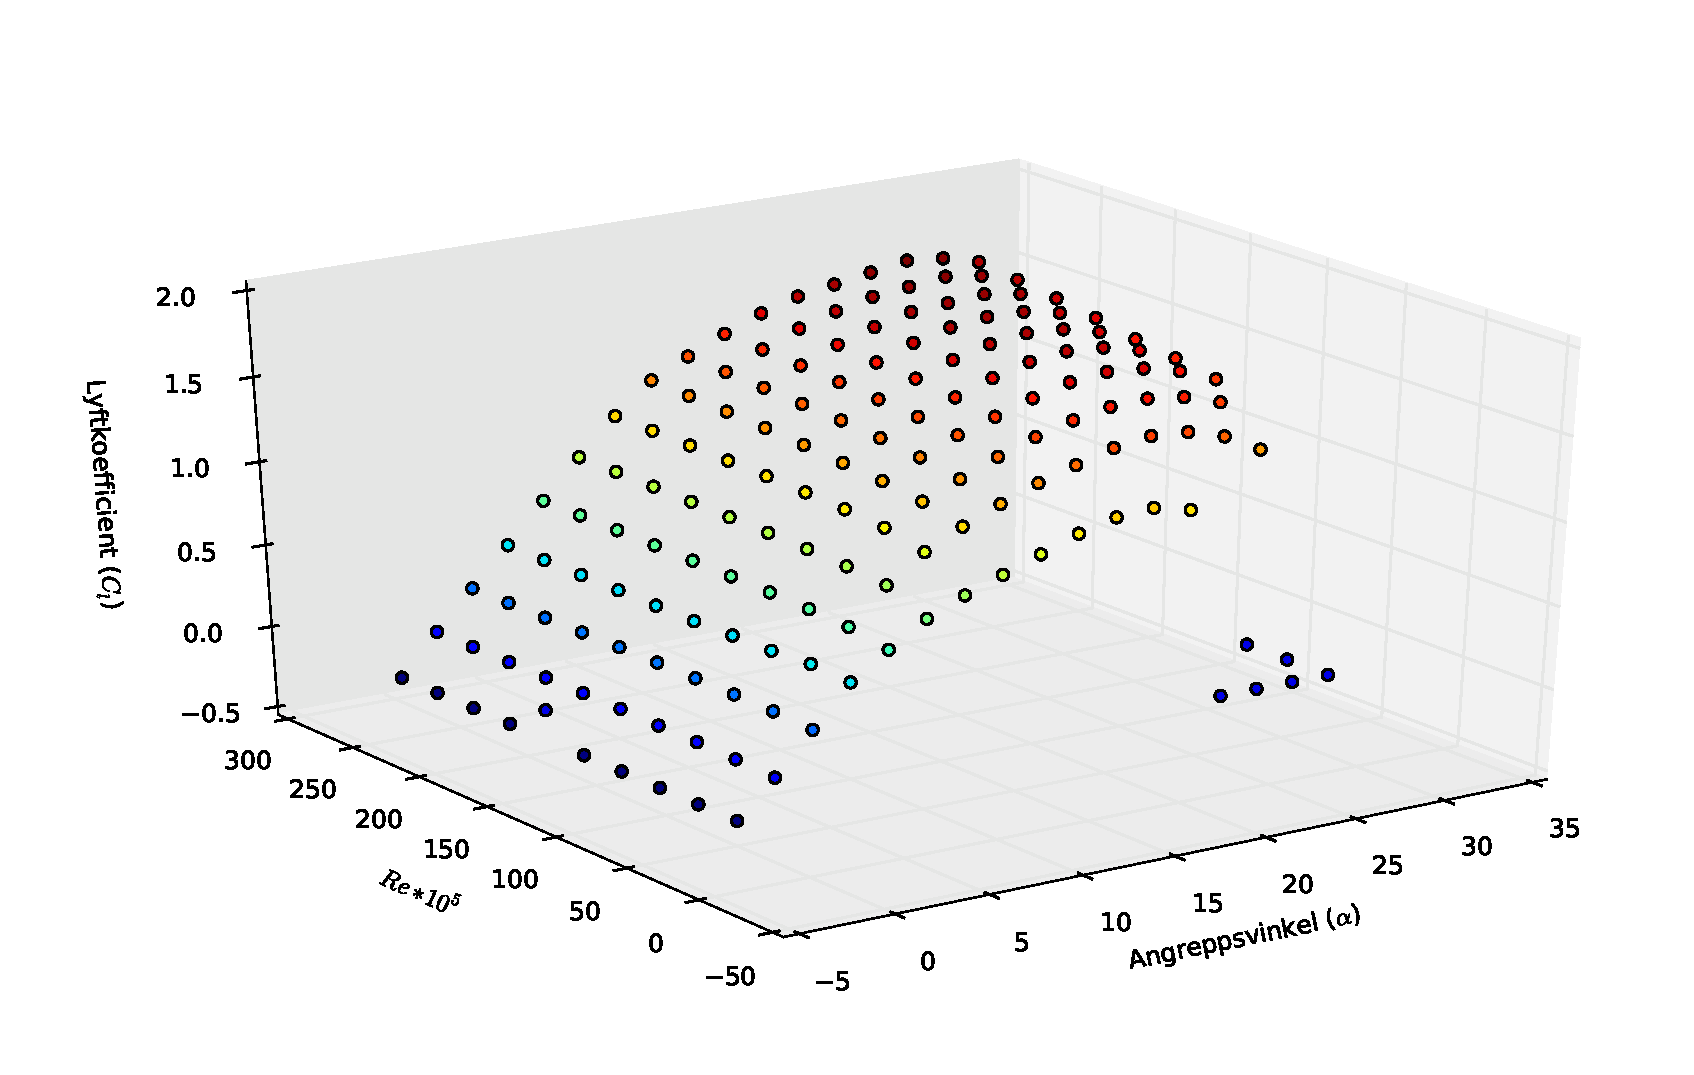
\includegraphics[width=1\textwidth]{Re_Alfa-map_scatter}
  \caption{Resulterande $C_l$ efter utvärdering av 10 st $Re$ i \textsc{Xfoil}}
  \label{xfoilscatter}
\end{figure}

\subsection{Hantering av uteblivet resultat från \textsc{Xfoil}}

För vissa $Re$ lyckas \textsc{Xfoil} inte ge något resultat över huvud taget. Detta hanteras genom att det problematiska $Re$ ignoreras och istället interpoleras mellanliggande fram som beskrivet i \ref{clinterpol}.

Det händer även att \textsc{Xfoil} låser sig. Exakt när detta sker och varför har inte kunnat kartläggas helt men beror förmodligen på en för avvikande vingprofil. För att kunna hantera detta har en timer implementerats. Har inget resultat kommit från \textsc{Xfoil} efter 60 sekunder får vingprofilen tilldelat sig negativa $C_l$ och $C_d$ för att på så sätt rensas ut.

\section{Post-stall-extrapolation av $C_d$ och $C_l$}
\label{post-stall}

\textsc{Xfoil} ger endast tillförlitliga resultat fram till $\alpha_{stall}$ \citep{XfoilVerifikation}. Av den anledningen har endast angreppsvinklarna $-5^{\circ} < \alpha < 30^{\circ}$ utvärderats med \textsc{Xfoil}. Därefter har $\alpha_{stall}$ satts till det $\alpha$ där $C_l$ haft högst värde ($C_{l_{stall}}$).

\textsc{Bem}-algoritmen behöver i vanliga fall inga $C_l$ och $C_d$ utanför  $-5^{\circ} < \alpha < \alpha_{stall}$. Men i undantagsfall och under optimeringsprocessen behövs $\alpha$ utanför intervallet. Därför har Viternaekvationerna implementerats vilka beskriver ett enkelt sätt att extrapolera $C_l$ och $C_d$ utanför intervallet. Detta beskrivs i \citet{viterna} och återges här i korthet.

Extrapoleringen av $C_d$ görs för intervallet $\alpha_{stall} < \alpha < 90^{\circ}$ görs med 

\begin{equation}\label{Cd} 
C_{d} = B_1\sin ^2\alpha + B_2\cos\alpha
\end{equation}

där 

\begin{subequations}
\label{ARB1B2}  
\begin{align}
        AR &= \frac{R}{c_{0.8R}}\\
        B_1 &= C_{d_{max}} = 1.11 + 0.018AR\\
        B_2 &= \frac{C_{D_{stall}}-C_{D_{max}}\sin^2\alpha_{stall}}{\cos\alpha_{stall}}
\end{align}
\end{subequations}

$AR$ är ett förhållande mellan radien och kordan ($c$) vid 80 \% av radien ($c_{0.8R}$). 

På liknande sätt kan $C_l$ extrapoleras i $\alpha_{stall} < \alpha < 90^{\circ}$ med

\begin{equation}\label{CL} 
C_l= A_1\sin2\alpha + A_2\frac{\cos^2\alpha}{\sin\alpha}
\end{equation}

där

\begin{subequations}
\label{A1A2}  
\begin{align}
        A_1 &= B_1/2\\
        A_2 &= (C_{l_{stall}}-C_{d_{max}}\sin\alpha_{stall}\cos\alpha_{stall})\frac{\sin\alpha_{stall}}{\cos^2\alpha_{stall}}
\end{align}
\end{subequations}

Ytterligare $C_l$ och $C_d$ kan extrapoleras med antagandet att vingprofilen beter sig som en platt platta i intervallet $ 90^{\circ} < \alpha < 180^{\circ}$ positivt och negativt


\begin{subequations}
\label{plattor} 
\begin{align}
        C_{L_{platta}} &= 2\sin\alpha\cos\alpha\\
        C_{D_{platta}} &= B_1\sin^2\alpha
\end{align}
\end{subequations}

Genom dessa ekvationer och datan från \textsc{Xfoil} kan nu $C_l$ och $C_d$ erhållas för $-180^{\circ} < \alpha < 180^{\circ}$. I \fref{clinterpolfig} syns datan från \textsc{Xfoil} i en tjockare blå linje medans den extrapolerade är den tunnare gröna linjen.

$C_d$ tas på samma sätt fram för hela spannet. I \fref{cdinterpolfig} syns \textsc{Xfoil}s data med tjock blå linje och den extrapolerade med tunn grön linje.


\begin{figure}[!h]
  \centering
  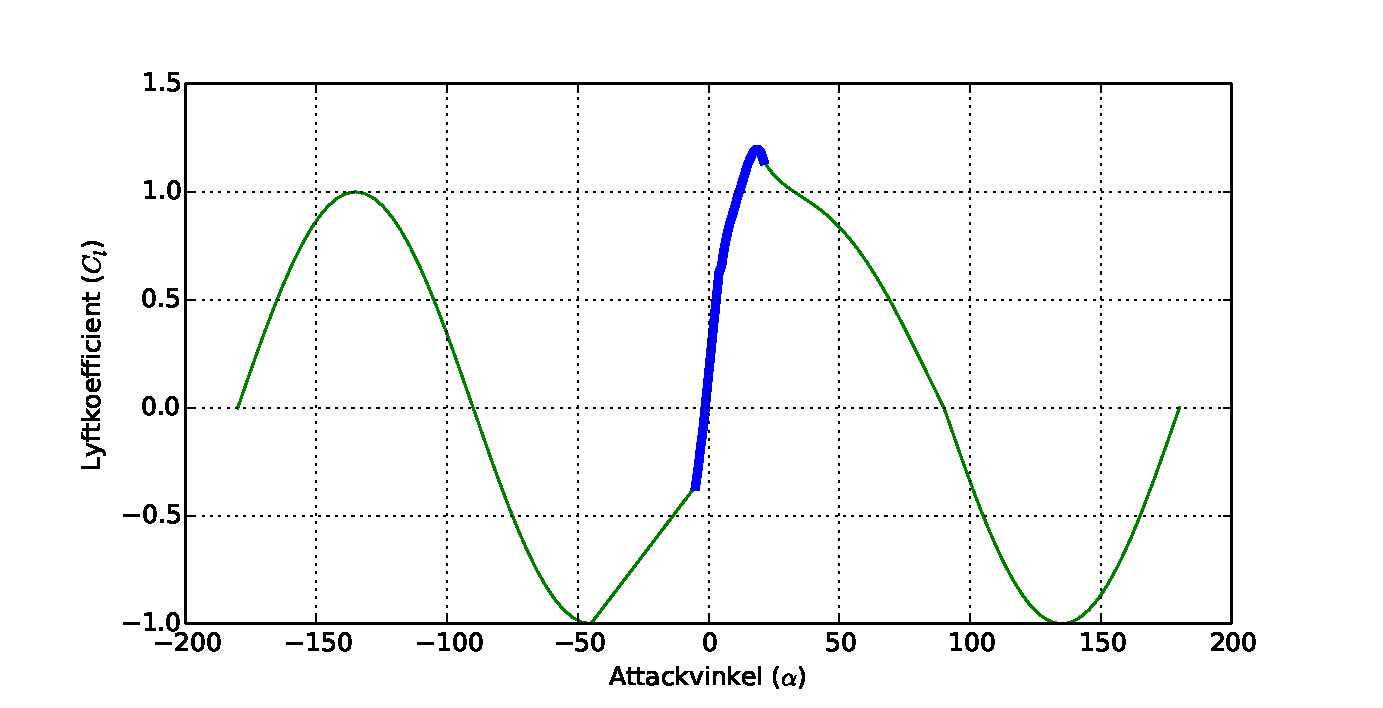
\includegraphics[width=0.9\textwidth]{liftinterpol}
  \caption{$C_l$ från \textsc{Xfoil} (fet linje) och extrapolerade $C_l$ (tunn linje) enligt förfarandet beskrivet i \ref{clinterpol} för en S809 vingprofil vid $Re$ en miljon. }
  \label{clinterpolfig}
\end{figure}


\begin{figure}[!h]
  \centering
  \includegraphics[width=0.9\textwidth]{draginterpol}
  \caption{$C_d$ från \textsc{Xfoil} (fet linje) och extrapolerade $C_d$ (tunn linje) enligt förfarandet beskrivet i \ref{clinterpol} för en S809 vingprofil vid $Re$ en miljon. }
  \label{cdinterpolfig}
\end{figure}







\section{Vindhastighetsprofiler}
\label{vindhastighetsprofiler}


SiteOpt tar som input en vindhastighetsprofil - det vill säga ett histogram över förekomsten av olika vindhastigheter för en plats. Data från St. Lawrence i Kanada \citep{Victoria} syns i \fref{vindprofil} (mätt 30 meter från marken). Antalet observationer har normerats till en procentuell förekomst. Summan av alla staplar är således 1.

Detta histogram används sedan i referensfallet och kallas vidare $h(U)$ (där $U$ är en vindhastighet) och används som uppskattning av den bakomliggande sannolikhetsfördelningen (vidare kallad $f_w(U)$). 

\begin{figure}[!htb]
  \centering
  \includegraphics[width=0.9\textwidth]{vindprofil}
  \caption{Vindhastighetsfördelning. Data från hämtad från St. Lawrence i Canada  reproducerad från \citet{Victoria}.}
  \label{vindprofil}
\end{figure}

\pagebreak

\section{Genetisk algoritm}

När den genetiska algoritmen initieras så skapas en första population. Denna utgår från vingprofilen S809 varpå de diskreta punkterna som bygger upp vingprofilen utsätts för en gaussisk slumpfaktor med standardavvikelse om 10 \% från de ursprungliga punkterna som bygger upp S809. Detta görs för att skapa en population med vingprofilskaraktär samtidigt som en bred del av designrymden söks av.

I \fref{initpop} visas den initiala populationens 28 första rot-vingprofiler som exempel, men populationen kan alltså även innehålla mellan-vingprofilen, top-vingprofilen, kordadistributionen och twistdistributionen som här ej visas. Dessa utsätts för samma slumpade initiering.

\begin{figure}[!htb]
\bigskip
  \centering
  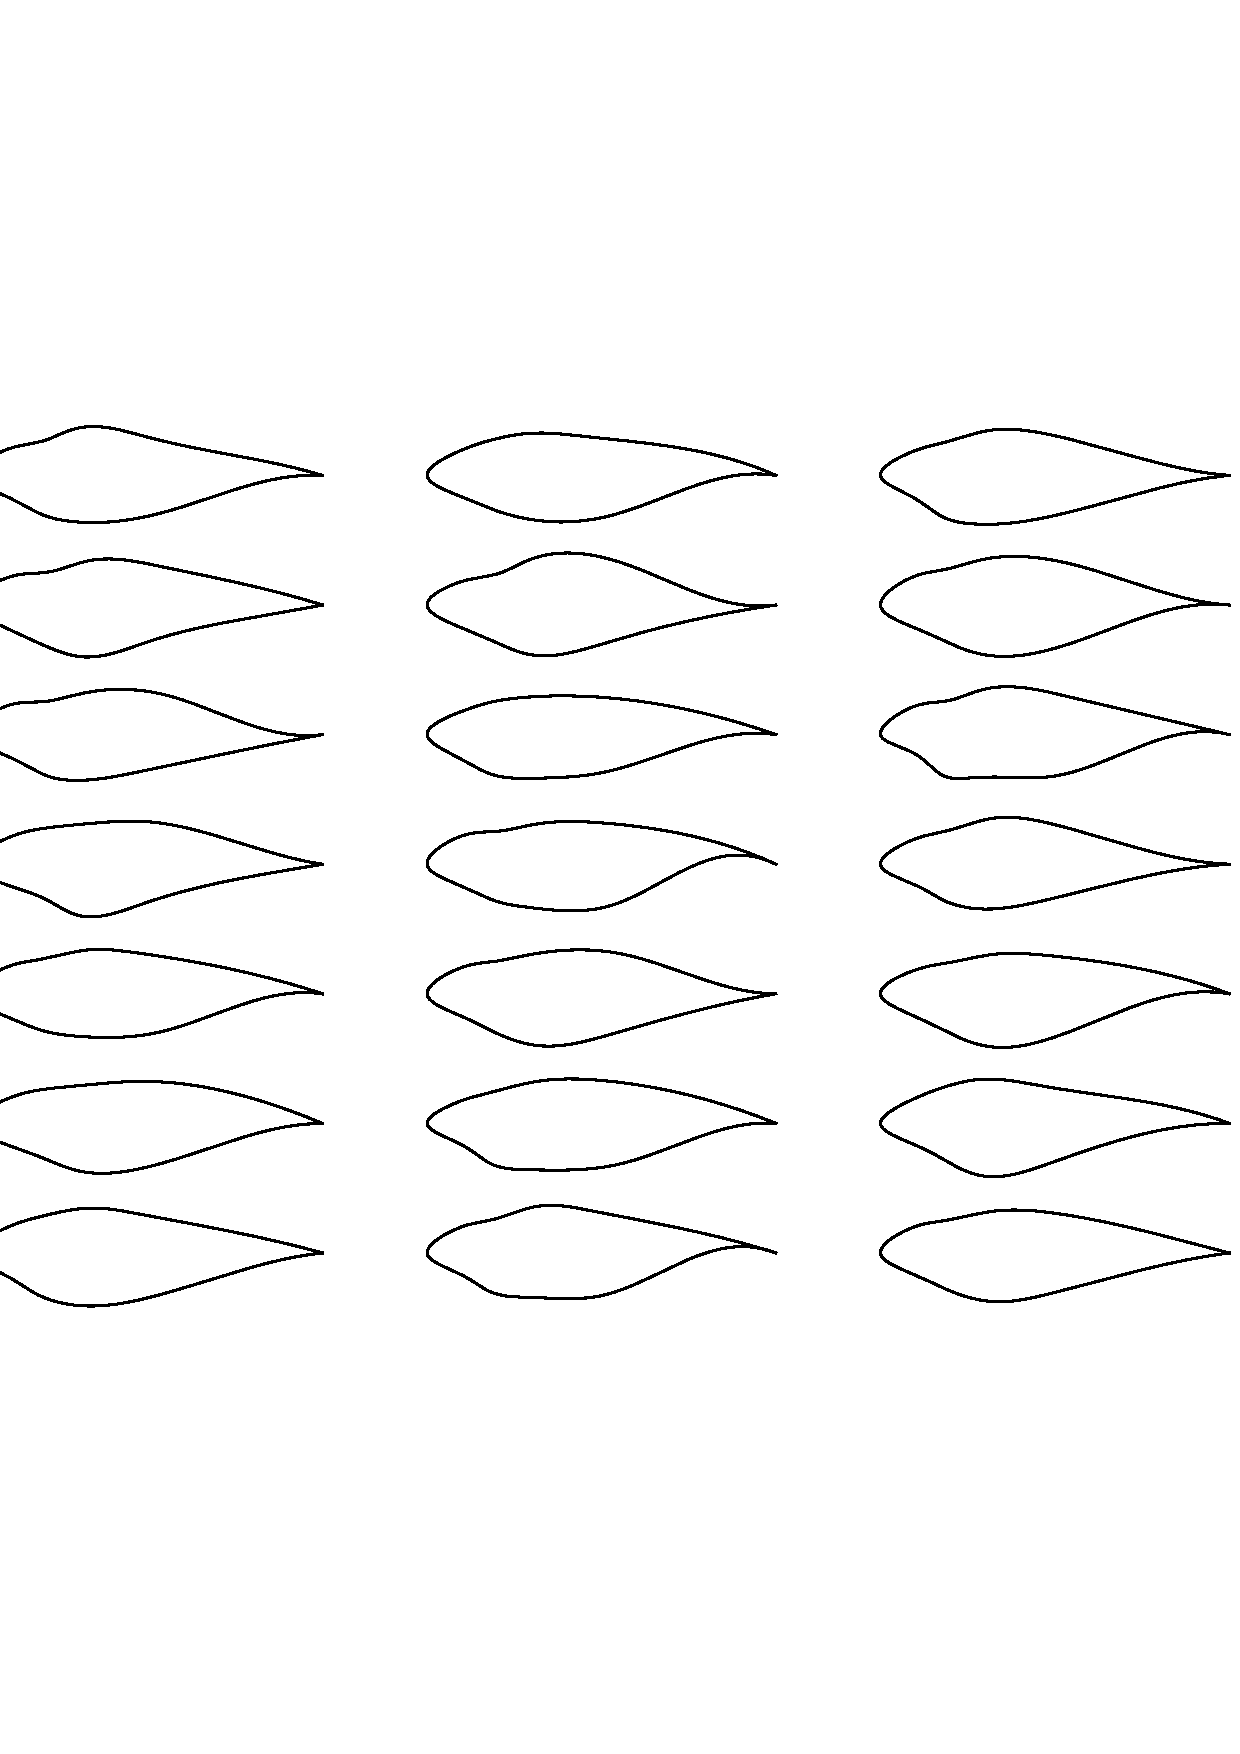
\includegraphics[width=1\textwidth]{initpop}
  \caption{Initial populations rot-vingprofiler skapad genom variationer på S809 med 10 \% slumpfaktor i varje punkt.}
  \label{initpop}
\end{figure}

\pagebreak

\subsection{Implementering av den genetiska algoritmen}

Biblioteket \textsc{Deap} till programmeringsspråket Python har använts med parametrar enligt \tref{GAparametrar} och algoritmen \lstinline[breaklines=true]!eaSimple!. Denna valdes eftersom det är en enkel implementation och trots litteraturstudien visat att mer avancerade algoritmer kan ge resultat till lägre beräkningskostnad. 


\bigskip
\begin{table}[!htb]
\small
  \centering
  
    \begin{tabular}{ll}
    
    \toprule
    Parameter & Värde \\
    \midrule
    Mutationssannolikhet för en individ ($MUT_{pb}) $ & 10 \%  \\
    Mutationssannolikhet för arvsmassans individuella element ($IND_{pb}) $ & 10 \%  \\
    Standardavvikelse för den gaussiska slumpfaktorn ($\sigma$) & 2 \% \\
    Sannolikhet att avkomma skapas genom korsning ($CX_{pb}$) & 50 \% \\
    Antal generationer innan avslut  ($N_G$)  & 10 000 st \\
    Populationsstorlek & 600 st \\
    \bottomrule
    \end{tabular}
  \caption{Parametrar för den genetiska algoritmen}
  \label{GAparametrar}
\end{table}

\bigskip
\vbox{%

 \lstinline[breaklines=true]!eaSimple! utsätter först en initial population för \emph{fitness-funktionen}. Efter detta påbörjas en generationsloop i vilken:
 
 
\begin{enumerate}
  \item Populationens individer utsätts för korsning med $CX_{pb}$ procents sannolikhet.
  \item De kvarvarande individerna utsätts för mutation enligt $MUT_{pb}$ procents sannolikhet där
  
  
  \begin{enumerate}
    \item arvsmassans element muteras med $IND_{pb}$ procents sannolikhet
    \item med en gaussisk avvikelse där standardavvikelsen är $\sigma$
  \end{enumerate}
  
  \item Alla individer skapade enligt ovan samt de kvarvarande orörda individerna överförs till nästa generation och processen återupprepas tills $N_G$ antal generationer passerat eller att användaren avslutar processen.
\end{enumerate}

} % end vbox

Förfarandet för  \lstinline[breaklines=true]!eaSimple! som i korthet här beskrivits återges mer utförligt i kapitel 7 av \citet{eaSimple}.




\pagebreak

\subsection{Fitnessfunktion}
\label{fitnessfunk}

\textsc{Bem}-metoden beskriven i \ref{siteoptBEM} ger alltså, givet en uppsättning vindhastigheter - en effektkurva. Denna kan med sannolikheterna för respektive vindhastigheter $h(U)$ (se \ref{vindhastighetsprofiler}) ge en genomsnittseffekt $\overline{P}$. Detta görs genom att sannolikhetsfördelningen $f_w$ aproximeras med vindhastighetshistogrammet $h(U)$ enligt

\begin{subequations}
\begin{align*}
        \overline{P} &= \int_{U_{in}}^{U_{ut}}f_w(U)P(U)dU \\
        &\approx  \sum_{U_{in}}^{U_{ut}} h(U)P(U)
\end{align*}
\end{subequations}

$\overline{P}$ ger nu approximativt hur pass bra ett vindkraftverk är för platsen som vidhistogrammet $h(U)$ beskriver eftersom summan av $h(U) = 1$.
